\documentclass[11pt,a4paper]{article}

\usepackage{fontspec}
\setmainfont{PT Serif}
\newfontfamily\headfont{PT Sans}
\usepackage[russian]{babel}
\usepackage[margin=2.2cm]{geometry}
\usepackage{booktabs}
\usepackage{graphicx}
\usepackage{xcolor}
\usepackage{array}
\usepackage{microtype}

\definecolor{accent}{HTML}{1f4e79}
\newcommand{\repsection}[1]{\vspace{0.6em}\noindent{\headfont\large\bfseries\color{accent}#1}\vspace{0.3em}\par}

\setlength{\parskip}{0.5em}
\setlength{\parindent}{0pt}
\pagenumbering{gobble}
% No Russian hyphenation patterns in this TeX install (basic scheme) -> allow
% extra interword stretch instead of overfull lines from unbreakable long words.
\sloppy

\begin{document}

{\headfont\Large\bfseries\color{accent} moex-backtest --- событийный бэктест-движок для MOEX}\\[0.2em]
{\headfont\large Пет-проект для перехода в quant-отдел}\\[0.3em]
\textit{Дмитрий Туминов, ВМК МГУ, 4 курс (кафедра ИО) $\cdot$ ML-разработчик, Финам $\cdot$ август 2026}

\vspace{0.5em}
\hrule
\vspace{0.8em}

\repsection{Что это}

Событийный (event-driven) бэктест-движок для российского рынка, написанный с нуля:
типизированный клиент MOEX ISS, модуль риск-метрик, движок исполнения с реалистичными
издержками и защитой от заглядывания вперёд (lookahead bias), пример торговой стратегии.
Инфраструктурный слой для последующего входа в Финам Арену: тот же интерфейс
стратегии, что используется здесь, можно будет подключить к Trade API вместо
симулятора без изменения кода стратегии.

\repsection{Архитектура}

\begin{itemize}
\itemsep0.15em
  \item \textbf{data} --- типизированный клиент MOEX ISS (пагинация, ретраи) + локальный parquet-кэш
  \item \textbf{metrics} --- Sharpe, Sortino, Max Drawdown, Calmar, историч. VaR/CVaR --- чистые функции
  \item \textbf{engine} --- цикл \texttt{Bar → Signal → Order → Fill}: Portfolio $\to$ SimulatedBroker $\to$ Backtester
  \item \textbf{strategy} --- интерфейс стратегии + baseline (buy \& hold) + пример (SMA-кроссовер)
\end{itemize}

\repsection{Инженерное качество}

\begin{itemize}
\itemsep0.15em
  \item \textbf{62 автотеста}, 99\% покрытие кода; \texttt{mypy --strict} и \texttt{ruff} --- без единого замечания
  \item \textbf{Защита от lookahead bias --- не соглашением, а конструкцией.} Сигнал,
        рассчитанный по цене закрытия бара $N$, исполняется по цене \emph{открытия} бара
        $N{+}1$ --- никогда раньше. Это зафиксировано отдельным тестом, а не оставлено
        на совесть автора стратегии
  \item \textbf{Издержки моделируются, а не игнорируются:} комиссия + проскальзывание на
        каждой сделке (см.\ раздел о влиянии издержек ниже)
\end{itemize}

\repsection{Находка при работе с MOEX ISS API}

Экспериментально (не из документации) установлено: анонимный доступ к истории
\emph{отдельных акций} ограничен $\sim$35 последними торговыми днями независимо от
запрошенного диапазона дат, тогда как история \emph{индексов} и \emph{опционов/фьючерсов
FORTS} такого ограничения не имеет. Это определило выбор инструмента для демонстрации
ниже (индекс, глубокая история) и задокументировано прямо в коде клиента.

\repsection{Результаты на реальных данных}

IMOEX, 2018-01-03 -- 2026-08-10 (2162 торговых дня), стартовый капитал 1\,000\,000~₽.
Комиссия 0.04\%, проскальзывание 5~б.п.\ на сделку, если не указано иное.

\begin{center}
\small
\begin{tabular}{lrrrrrrr}
\toprule
Стратегия & Дох.\ год.\ & Волат.\ & Sharpe & Sortino & MaxDD & Calmar & Сделок \\
\midrule
Buy \& Hold                    & 0.7\%  & 25.3\% & 0.03 & 0.03 & $-$55.3\% & 0.01 & 5 \\
SMA(10,50)                     & 3.2\%  & 12.1\% & 0.26 & 0.19 & $-$29.2\% & 0.11 & 140 \\
SMA(20,100)                    & 2.1\%  & 12.8\% & 0.17 & 0.12 & $-$27.5\% & 0.08 & 83 \\
SMA(50,200)                    & 2.1\%  & 13.3\% & 0.16 & 0.11 & $-$36.2\% & 0.06 & 29 \\
\midrule
SMA(20,100), без издержек\textsuperscript{*} & 2.4\% & 12.8\% & 0.19 & 0.13 & $-$27.4\% & 0.09 & 83 \\
\bottomrule
\end{tabular}
\end{center}

\footnotesize\textsuperscript{*}~Иллюстративное сравнение: тот же прогон с нулевой
комиссией и проскальзыванием --- показывает, что реалистичные издержки съедают
$\sim$0.02--0.03 пункта Sharpe при 83 сделках за 8.5 лет.
\normalsize

Все стратегии --- long-only, взвешивание по целевой доле капитала (без плеча).
SMA-кроссовер --- заведомо простая учебная стратегия для проверки движка, не
претендует на реальный alpha.

\repsection{Кривая капитала}

\begin{center}
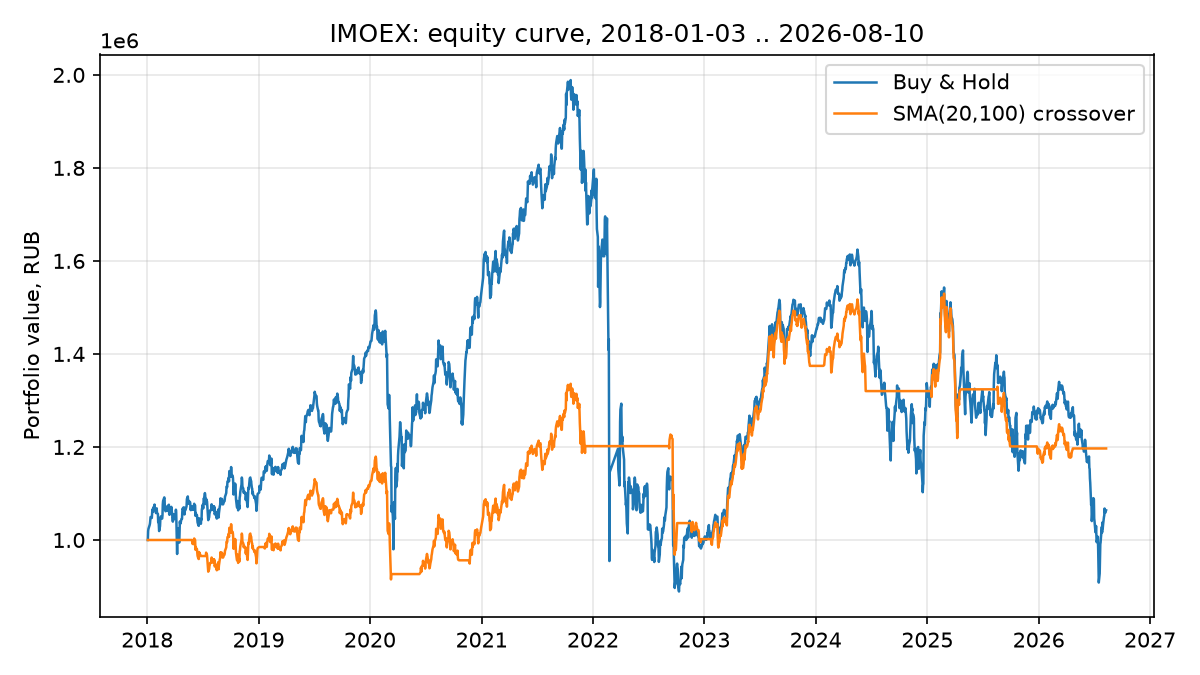
\includegraphics[width=0.92\textwidth]{assets/equity_curve.png}
\end{center}

\vspace{-0.3em}
\footnotesize
Заметно на графике: SMA-кроссовер почти не участвует в обвале начала 2022 года
(резкое падение индекса) и в целом даёт более плоскую кривую капитала ценой меньшего
участия в ралли 2020--2021 --- типичный компромисс trend-following стратегий между
просадкой и апсайдом.
\normalsize

\repsection{Дальше}

\begin{itemize}
\itemsep0.15em
  \item Мультиактивный портфель с риск-лимитами по CVaR --- естественное продолжение
        риск-ориентированного подхода из курсовой работы (Kalman-фильтр, адаптивное
        сглаживание, CVaR/MDD в награде RL)
  \item Адаптер исполнения через Финам Trade API --- тот же интерфейс \texttt{Strategy}
        сможет торговать в Финам Арене без изменения кода стратегии
  \item Стратегия с реальным edge --- нынешний SMA-кроссовер существует, чтобы
        проверить движок целиком, не для реальной торговли
\end{itemize}

\end{document}
